%%%%%%%%%%%%%%%%%%%%%%%%%%%%%%%%%%%%%%%%%%%%%%%%%%%%%%%%%%%%%%%%%%%%%%%%
% Copyright (c) 2022 Antonio Coín
%
% This work is licensed under a
% Creative Commons Attribution-ShareAlike 4.0 International License.
%
% You should have received a copy of the license along with this
% work. If not, see <http://creativecommons.org/licenses/by-sa/4.0/>.
%%%%%%%%%%%%%%%%%%%%%%%%%%%%%%%%%%%%%%%%%%%%%%%%%%%%%%%%%%%%%%%%%%%%%%%%

%%%%%%%%%%%%%%%%%%%%%%%%%%%%%%%%%%%%%%%%%%%%%%%%%%%%%%%%%%%%%%%%%%%%%%%%
\chapter{Introduction}\label{ch:introduction}
%%%%%%%%%%%%%%%%%%%%%%%%%%%%%%%%%%%%%%%%%%%%%%%%%%%%%%%%%%%%%%%%%%%%%%%%

Over the last few decades, situations involving data in the form of functions have become commonplace in many statistical scenarios, as more and more information is available worldwide with an ever-increasing level of granularity in the measurements. In particular, functional data problems are far from unheard of in the data science an machine learning community, since they have attracted the attention of researchers and practitioners equally. Medical data, weather indicators or stock exchange indices are examples of elements that benefit from a functional treatment, where the observations are regarded as single entities rather than as a conglomerate of individual points.

Under a functional framework, the objects of interest are \textit{random functions} instead of random points in a finite-dimensional space. While in principle the functional data could be simply regarded as a discretized vector in a very high dimension (an indeed such a discretization is performed in practice), there are often many advantages in taking into account the functional nature of the data, ranging from modeling the possibly high correlation among points that are close in the domain, to extracting information that may be hidden in the derivatives of the function in question. Thus, the general idea is to assume the existence of an underlying sufficiently smooth function that generates each (possibly noisy) functional observation, even though we only record it on a finite grid of points.

To see what this kind of data looks like, Figure~\ref{fig:tecator_orig} shows an example of a functional data set, which is known in the literature as the Tecator data set, and whose elements represent near-infrared absorbance curves of meat samples. The objective here is to predict the fat content based on this absorbance spectrum, separating the samples into those with ``high'' and ``low'' fat content. At first glance it does not seem that the trajectories contain much relevant information to help classify the samples. However, after a suitable smoothing of the data (e.g. by representing each function in a Fourier basis) we can take the derivatives of the curves. In this case, after differentiating twice a clearer pattern emerges (see Figure~\ref{fig:tecator_derivatives}), one from which inference and prediction will surely be easier.

\begin{figure}[ht!]
  \begin{subfigure}[b]{0.48\textwidth}
    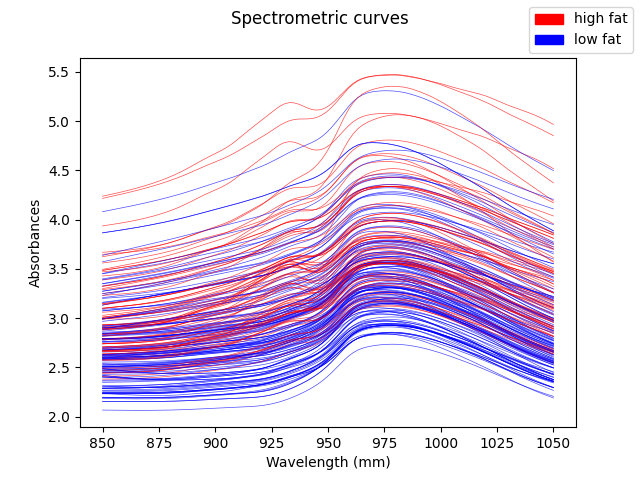
\includegraphics[width=\textwidth]{tecator}
    \caption{Original curves}\label{fig:tecator_orig}
  \end{subfigure}
  \hfill
  \begin{subfigure}[b]{0.48\textwidth}
    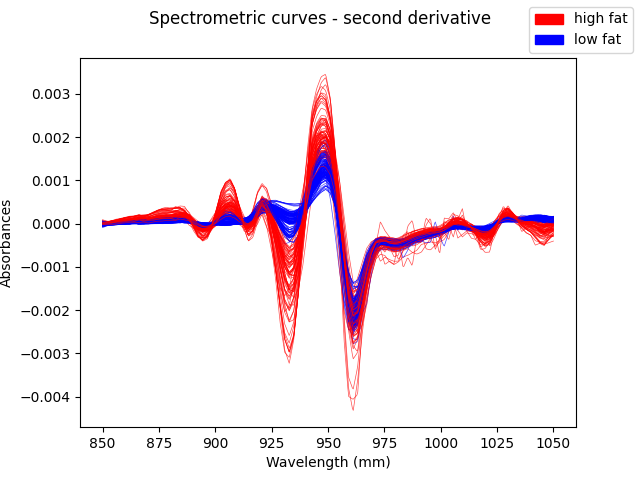
\includegraphics[width=\textwidth]{tecator_derivative}
    \caption{Second derivatives}\label{fig:tecator_derivatives}
  \end{subfigure}
  \caption{Curves in the Tecator data set and their second derivatives (after smoothing).}\label{fig:tecator}
\end{figure}

In recent years numerous proposals have arisen on how to suitably deal with functional data, all of them encompassed under the term Functional Data Analysis (FDA), which essentially explores statistical techniques to process, model and make inference on data varying over a continuum. A partial survey on such techniques and methods is \citet{cuevas2014partial}, while a more detailed exposition of the theory and applications can be found for example in \citet{hsing2015theoretical} or the book by \citet{horvath2012inference}. As the name suggests, FDA techniques are heavily inspired by functional analysis tools and methods: Hilbert spaces, orthonormal systems, linear operators, and so on. In particular, a notion that also intersects with the classical theory of machine learning and pattern recognition is that of reproducing kernel Hilbert spaces (RKHS's). We will demonstrate throughout this work how these spaces of functions possess properties that allow for an efficient treatment of functional data. On the other hand, Bayesian inference methods are ubiquitous in the realm of statistics, and their usual non-parametric approach also makes use of random functions, though in a slightly different manner than in the FDA context. However, the two methodologies can certainly interact and benefit from one another, as we intend to show in this thesis. We will be particularly interested in Markov chain Monte Carlo (MCMC) methods, which allow us to approximate an arbitrary posterior distribution through a function proportional to its density.

\begin{center}
\color{teal}\FourStar
\end{center}

In this work we are concerned with functional linear and logistic regression models, that is, situations where the goal is to predict a continuous or dichotomous variable from functional observations. Even though these problems can be formally stated with almost no differences from their finite-dimensional counterparts, there are some fundamental challenges as well as some subtle drawbacks that emerge as a result of working in infinite dimensions. Moreover, we will concentrate our efforts on the case in which the response is a scalar, though function-on-function and function-on-scalar regression are also interesting scenarios amply explored in the literature. To set a common framework, throughout this work we will consider a scalar response variable \(Y\) (either continuous or binary) which has some dependence on a stochastic \(L^2\)-process \(X=X(t)=X(t, \omega)\) with trajectories in \(L^2[0, 1]\) (i.e. a process with finite second moments and whose realizations are square-integrable functions indexed on \([0,1]\)). The underlying probability space \((\Omega, \mathcal A, \P)\) is not important. We will further suppose without loss of generality that \(X\) is centered, that is to say, its mean function \(m(t)=\E[X(t)]\) vanishes for all \(t\in[0,1]\). In addition, we will tacitly assume the existence of a \textit{labeled} data set \(\D_n =\{(x_i, y_i): i=1,\dots, n\}\) of independent observations from \((X, Y)\), where the functional observations are recorded on a common finite grid \(\{t_j\}\subset [0, 1]\). Our ultimate aim will be to accurately predict the response corresponding to unlabeled samples from \(X\). Figure~\ref{fig:linear_data_example} depicts a typical data set used in functional regression, and we already saw in Figure~\ref{fig:tecator} what a functional classification data set may look like.

\begin{figure}[ht]
  \centering
  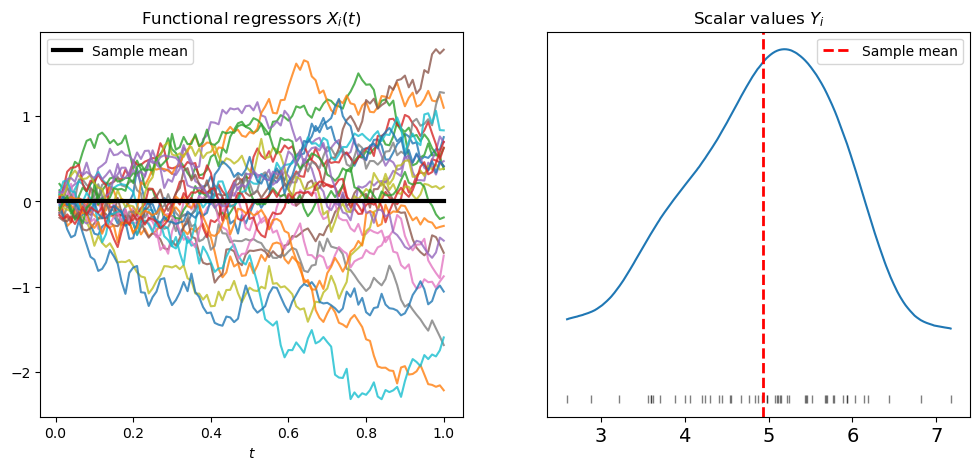
\includegraphics[width=0.9\textwidth]{linear_data_example}
  \caption{Simulated data set for functional regression. On the left we have \(n=50\) functional observations on an equispaced grid of \(N=100\) points on \([0,1]\). To each observation corresponds a real number; the distribution of these responses is shown on the right.}\label{fig:linear_data_example}
\end{figure}


\section{Objectives and scope}

We list below the main objectives of this work in no particular order.

\begin{enumerate}[1.]
  \item To perform a brief but thorough literature review that contextualizes functional linear and logistic regression within statistics and machine learning, exploring the predominant models and techniques.
  \item To propose a novel RKHS-based functional model for linear and logistic regression that builds on existing work and focuses on simplicity, both in terms of interpretation and implementation.
  \item To describe and implement a general Bayesian approach for parameter estimation within the suggested model.
  \item To introduce the tools needed to specify the proposed model and put it into practice, mainly reproducing kernel Hilbert spaces and Markov chain Monte Carlo methods.
  \item To carry out an extensive experimental study to test these new models and compare them to existing methods, both in simulations and in real-world scenarios.
\end{enumerate}

It is beyond the scope of this thesis to provide a complete review of FDA as a whole, or to delve too deeply into the details and inner workings of most models and techniques mentioned. Nevertheless, references are provided frequently throughout the text to point the interested reader towards more specialized resources.

\section{Structure overview}

In Chapter~\ref{ch:background} we summarize the relevant literature related to our problem, along with a review of the basics of RKHS's and MCMC methods. Chapter~\ref{ch:bayesian} is devoted to explaining the Bayesian methodology and the functional regression models we propose. Then, in Chapter~\ref{ch:model-choice} we present a short discussion of theoretical and computational details that have led to the concrete specification of the model, as well as some validation techniques. The empirical results of the experimentation are contained in Chapter~\ref{ch:experiments}. Lastly, the conclusions drawn from this work and future paths of research are reviewed in Chapter~\ref{ch:conclusions}.
